\subsection{Results}
% -------------------------------------------------------------------------
Particle neighborhoods created with the Delaunay edge detection algorithm
are used to correct the over-segmented results
(\ref{fig/05/merge-results}.b) obtained from the watershed
segmentation. The regions corresponding to each of the markers within a
particle neighborhood are merged such that each particle neighborhood has
only one associated region in the final segmented regions
(\ref{fig/05/merge-results}.c).

\begin{figure}[ht]
    \centering
    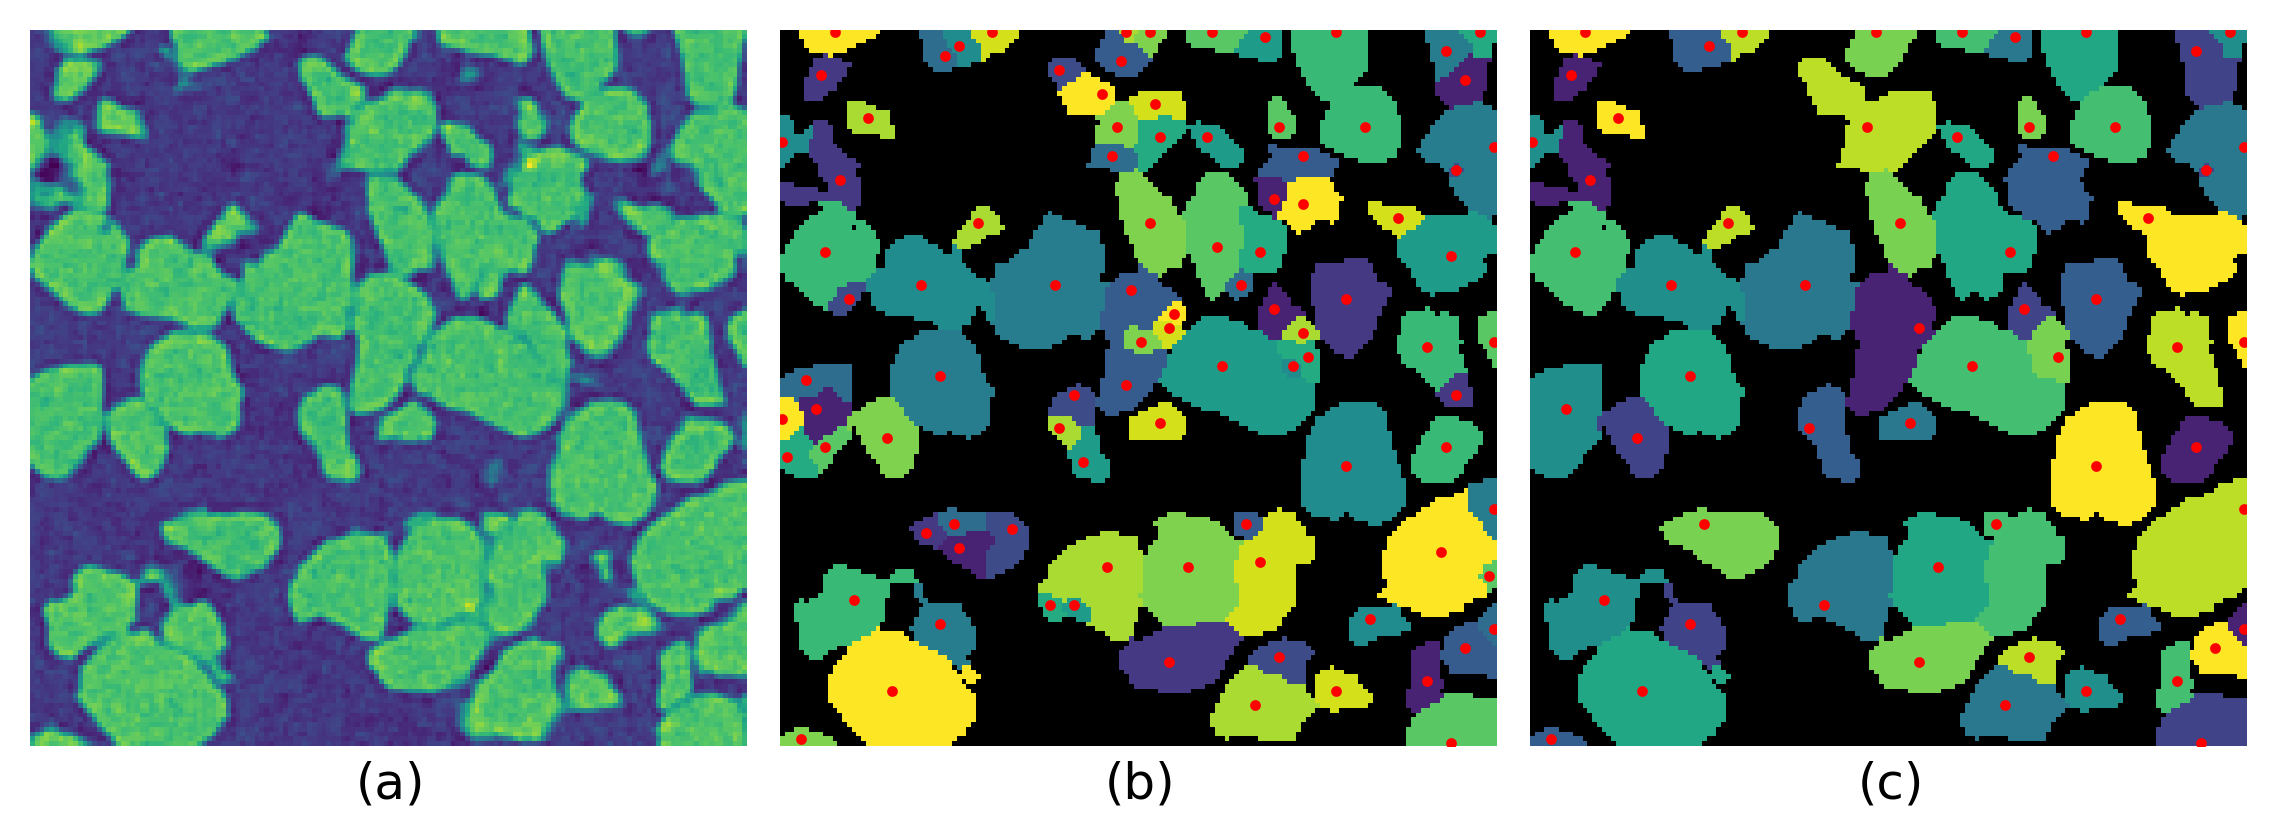
\includegraphics[width=0.75\textwidth]{figures/05/08-seg-results.png}
    \caption{
        \small\setstretch{1}
        (a) Image depicting sand particles to compare with segmentation
        results.
        (b) Over-segmented regions resulting from extended watershed routine,
        but before regions are merged (\ref{fig/05/overseg}.c).
        Red points correspond to marker used to segment the region.
        (c) Final segmented regions after merging neighboring regions without
        a separating edge (\ref{fig/05/delaunay}.b). Each red point
        corresponds to the marker of a merged region closest to the average
        location of all the centroids of the merged neighboring regions.
    }
    \label{fig/05/merge-results}
\end{figure}

The merging algorithm yields a segmentation that appears to more closely align with
expectations than the results from a typical watershed segmentation when
compared to the visually discernible grains in the original image
(\ref{fig/05/merge-results}.a). However,
in order to quantitatively determine the extent to which the merging algorithm
improves the results obtained from the watershed segmentation, the results from
the typical watershed and merged-region segmentations are compared to a manual
segmentation of the sand grains.
To generate the manual segmentation, a digital drawing application
with multi-layer functionality was used to individually draw the footprint of
each segmented grain on a separate layer overlaid on the raw image.
Each layer was then exported as a separate PNG image. These images were loaded into
Python using \textit{imageio} and \textit{NumPy}, and the grain in each
labeled image was assigned a unique integer ID using \textit{scikit-image}.

It is nontrivial to calculate the fit between two separate segmented images, even
though the images both represent the same system. Even when labeled regions are
relatively closely aligned, the labels in each segmented image will most likely not
match. To solve this problem, an algorithm was written to match the labels across two
separately segmented images based on maximum overlapping area without
reusing any labels. This allowed for a match value to be calculated by summing the
overlapping matching pixels and dividing by the sum of all pixels, matched and
mismatched. Using this method,
a match of 82.09\% was calculated between the manual segmentation and the
typical watershed segmentation,
whereas a match of 89.02\% was calculated between the manual
segmentation and the merged-region segmentation.

